\documentclass{acmart}
\usepackage{amsmath}
\usepackage{amsfonts}
\usepackage[utf8]{inputenc}
\newcommand{\x}{\mathbf{x}}
\usepackage{float}
\usepackage{graphicx}
\usepackage{subcaption}

\AtBeginDocument{%
  \providecommand\BibTeX{{%
    \normalfont B\kern-0.5em{\scshape i\kern-0.25em b}\kern-0.8em\TeX}}}

 \citestyle{acmauthoryear}
\graphicspath{{figures/}}

%%
\title{Leveraging Weighted Sums for Integrating Message-Passing and Global Attention in GPS Graph Transformer}
\author{Tal Ben Tov - 208634766}
\author{Omer Talmi - 318900883}
\author{Lia Soffer - ID}

\date{}

\begin{document}

\begin{abstract}
TL;DR of this project - one paragraph
\end{abstract}
\maketitle
\footnotetext[1]{Code is publicly available at \url{https://github.com/omertalmi5/WeightedGraphGPS }.}

\section{Introduction}

Graph Neural Networks (GNNs) have become a key paradigm for modeling relational data across numerous applications, including social network analysis, chemical graph prediction, and recommendation systems \cite{gilmer2017neuralmessagepassingquantum}. Among the most widely studied GNN variants are \textbf{Message Passing Neural Networks (MPNNs)}, which aggregate information from node neighbors through iterative message-passing steps. MPNNs have been shown to excel at capturing local graph structures, making them well-suited for tasks such as molecular property prediction and community detection in social networks \cite{gilmer2017neuralmessagepassingquantum}. However, MPNNs struggle to capture long-range dependencies due to over-squashing \cite{alon2021bottleneckgraphneuralnetworks} and often suffer from high locality bias due to over-smoothing \cite{oono2021graphneuralnetworksexponentially}, limiting their performance on tasks requiring global information flow \cite{dwivedi2022benchmarkinggraphneuralnetworks}.


On the other hand, \textbf{Graph Transformers (GTs)} were introduced to address these limitations by incorporating global attention mechanisms. Transformers in the graph domain allow nodes to attend to all other nodes in the graph, making them highly effective at alleviating over-smoothing and over-squashing \cite{alon2021bottleneckgraphneuralnetworks, topping2022understandingoversquashingbottlenecksgraphs}. The attention mechanism enables nodes to focus on more distant regions of the graph, alleviating issues of locality and improving the expressiveness of the model \cite{xu2019powerfulgraphneuralnetworks, morris2021weisfeilerlemanneuralhigherorder}. However, a major drawback of GTs lies in their quadratic computational complexity $\mathcal{O}(N^2)$ for a graph with $N$ nodes and $E$ edges \cite{vaswani2023attentionneed}, which can be prohibitive for large-scale graphs commonly encountered in real-world tasks like traffic systems or genomic analysis \cite{dwivedi2022benchmarkinggraphneuralnetworks}.

To strike a balance between local processing in GNNs and global attention in GTs, the \textbf{General, Powerful, and Scalable (GPS) framework} was proposed \cite{rampášek2023recipegeneralpowerfulscalable}. GPS combines the best of both worlds by applying a message-passing layer to capture local information and a global attention layer to capture long-range dependencies in each layer of the model. This alternating structure allows GPS to efficiently process graphs while maintaining the benefits of both MPNNs and GTs. However, while GPS successfully integrates local and global mechanisms, the fixed alternation between message-passing and global attention layers may not always be optimal for every graph structure, as some graphs may require more attention on local interactions, while others might benefit from global connectivity patterns \cite{Bronstein_2017}.

In this work, we propose a novel approach to dynamically scale between the local message-passing and global attention layers within the \textbf{GPS} architecture. Instead of a fixed alternation between layers, we introduce a scaling mechanism that computes a weighting vector to scale the contribution of each layer based on node-level features. This adaptive weighting aims to:

\begin{itemize}
    \item \textbf{Improve the performance} of the GPS framework by tailoring the balance between local and global information to the specific characteristics of the graph.
    \item \textbf{Understand the conditions} under which global attention or message-passing is more effective by analyzing the learned weights across diverse types of graphs. For instance, in certain molecular graphs, local interactions between nearby atoms may dominate, whereas in social networks, the ability to model long-range dependencies could be crucial.
\end{itemize}

By investigating the scaling weights learned for different graphs, we aim to uncover properties of graphs, such as \textbf{density, connectivity, community structure, and long-range correlations}, that influence the relative importance of local versus global mechanisms. This approach offers insights into how MPNN and Transformer components can be optimally combined in a single model to achieve better performance across diverse graph datasets.

\section{Related Work}

Recent studies have further explored hybrid models that integrate MPNN-based message-passing and Transformer-based global attention. For instance, in molecular property prediction tasks, hybrid models like \textbf{Graphormer} \cite{ying2021transformersreallyperformbad, shi2023benchmarkinggraphormerlargescalemolecular} have shown that combining MPNN and Transformer components leads to superior performance by capturing both local molecular interactions and global structural motifs. Graphormer improves Transformer performance on molecular graphs by introducing a spatial encoding that preserves the inherent structure of graphs while leveraging attention \cite{vaswani2023attentionneed, gilmer2017neuralmessagepassingquantum}.

Similarly, \textbf{SAN (Graph Structure-Aware Transformer)} \cite{kreuzer2021rethinkinggraphtransformersspectral} enhances standard Transformers by incorporating structural information into the attention mechanism, enabling the model to account for graph connectivity while processing global attention. These models demonstrate that combining local and global mechanisms can significantly improve expressiveness and performance in diverse domains, particularly for tasks where long-range dependencies are critical, such as molecular dynamics or large-scale social network analysis.

In the GPS framework \cite{rampášek2023recipegeneralpowerfulscalable}, the MPNN and global attention layers are combined through a summing-up approach, where the output of the message-passing layer is added to the output of the global attention layer at each iteration. This additive approach offers several benefits. First, it allows the model to capture both local and global information simultaneously, leveraging the strengths of MPNNs in encoding neighborhood structures and the ability of attention mechanisms to capture long-range dependencies. By summing these outputs, GPS ensures that both types of information contribute equally to the final node embeddings without one mechanism overpowering the other. This balance helps mitigate issues like over-smoothing, which can occur if MPNN layers dominate \cite{oono2021graphneuralnetworksexponentially}, or computational complexity, which arises from relying solely on attention layers \cite{vaswani2023attentionneed}. Moreover, the additive fusion avoids excessive model complexity, keeping the architecture simple yet powerful, which is particularly useful in large-scale graphs where computational efficiency is critical.

However, challenges remain in such hybrid systems, including the GPS framework. The use of both MPNN and Transformer layers often introduces \textbf{model complexity}, requiring careful tuning of hyperparameters to balance local and global components \cite{rampášek2023recipegeneralpowerfulscalable}. Moreover, certain tasks may disproportionately rely on local or global information, making it difficult to generalize the relative importance of each component across different datasets.

\section{Method}

In this paper, we propose a novel architecture where each layer consists of two parallel components: a message-passing layer and a global attention layer. Instead of summing them sequentially as in GPS, we compute a weighted sum of their outputs using learned weights throughout the layers. This is done by incorporating a dynamic gating mechanism based on node-level features. This allows the model to decide at each layer the relative importance of message passing versus global attention per node.

\subsection{Dynamic Gating Network Design}

The core innovation of this work lies in the introduction of a dynamic gating network within the GPS layer. The gating network consists of two GCNConv layers, where the first layer reduces the dimensionality of node features, and the second layer outputs two gating scalars for each node. These scalars are passed through a softmax function.

Thus, the network learns the optimal scaling coefficients for each node based on the graph structure, allowing the GCNConv to balance the contributions of local message passing and global attention dynamically.

The softmax has multiple roles. 

First, it ensures that the combined weights for the local and global representations sum to 1, thereby providing a normalized weighting scheme. 

More importantly, the softmax mechanism allows the network to dynamically choose between the two modalities (local and global) by assigning a higher weight to the more relevant representation in each context. Unlike a simple averaging or summation of the representations, the softmax emphasizes the better one for the given input by selectively amplifying the scalar corresponding to the dominant modality. This dynamic selection ensures that the GPS layer is context-aware and capable of prioritizing either message passing (local) or global attention (global), depending on the specific requirements of the node’s environment.

In mathematical terms, the scalars of the $\ell$-th layer are computed as:

\begin{equation}
\mathbf{a}_{\text{mag}}^{\ell}, \mathbf{a}_{\text{attn}}^{\ell} = \text{softmax}\left(\text{GCNConv}_2\left(\text{ReLU}\left(\text{GCNConv}_1(\mathbf{h}^{\ell})\right)\right)\right)
\end{equation}


Here, \( \mathbf{a}_{\text{M}}^{\ell} \) and \( \mathbf{a}_{\text{T}}^{\ell} \) are the gating scalars corresponding to the message passing and global attention mechanisms, respectively. h is initially the node features, and then is updated by the rule:

\[
\mathbf{h}^{\ell+1} = \mathbf{a}_{\text{mag}}^{\ell} \cdot \mathbf{h}_{\text{local}}^{\ell} + \mathbf{a}_{\text{attn}}^{\ell} \cdot \mathbf{h}_{\text{attn}}^{\ell}
\]

Here, $\mathbf{h}_{\text{local}}^{\ell}$ represents the node features obtained from local GNN-based message-passing, and $\mathbf{h}_{\text{attn}}^{\ell}$ represents the node features obtained from the global attention mechanism. The scalar outputs dynamically adjust the importance of the local and global representations at the node level.

The softmax ensures these scalars are non-negative and sum to 1, promoting competition between them to emphasize the stronger signal. This formulation allows the GPS layer to leverage the most appropriate mechanism—whether it is graph-based message passing or transformer-style attention—depending on the specific input characteristics and graph topology.


The method's advantage lies in its flexibility—by dynamically adjusting the contributions of local and global information for each node, the model can adapt to a wide variety of graph structures and tasks. The experimental setup follows the GPS framework, leveraging both small- and large-scale graph benchmarks to demonstrate the scalability and effectiveness of the proposed method.

\begin{figure}[ht]
  \centering
  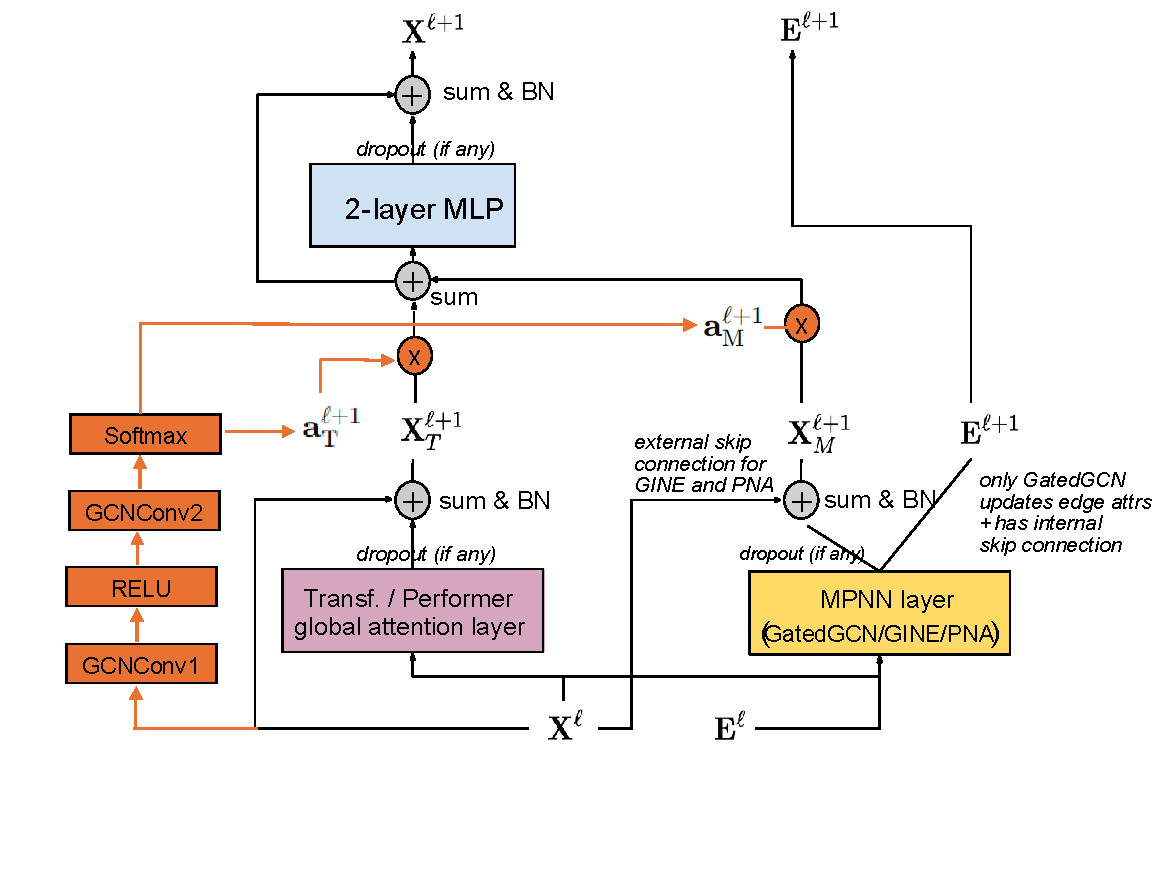
\includegraphics[width=1\textwidth]{WGPS-layer}
  \caption{The WGPS layer, with modifications from the original GPS layer showed in orange: In the $({\ell}+1)$-th layer, the dynamic gating network outputs two scalars, $a_T^{{\ell}+1}$ and $a_M^{{\ell}+1}$, which are used to compute a weighted sum between the node features $X_T^{{\ell}+1}$ and $X_M^{{\ell}+1}$, obtained after passing through the Global Attention and MPNN layers, respectively: $a_M^{{\ell}+1} \cdot X_M^{{\ell}+1} + a_T^{{\ell}+1} \cdot X_T^{{\ell}+1}$.
}
  \label{fig:wgps_layer}
\end{figure}

\section{Experiments and Results}
Describe in detail the experiments you conducted, the datasets you used, the evaluation metrics, and models or other methods you compared against. Explain how you generated your splits or where you obtained them. Make sure to explain every experiment you show: what is the goal of this experiment? If needed, include running time or memory usage reports.

This is also the place to include details on your implementation, such as which libraries you used, and a link to a public GitHub repository with the code (can be an anonymous GitHub) - 1-2 pages.

\subsection{Datasets}
We utilize datasets from both the Benchmarking GNNs \cite{dwivedi2022benchmarkinggraphneuralnetworks} and the Open Graph Benchmark (OGB) \cite{hu2021opengraphbenchmarkdatasets}. From Benchmarking GNNs, we employ the ZINC dataset, and from OGB we employ three graph-level datasets: ogbg-molhiv, ogbg-molpcba and ogbg-code2 / ogbg-ppa.

\begin{table}[htbp]
\centering
\caption{Summary of the graph learning datasets utilized in this paper.}
\begin{tabular}{|l|c|c|c|c|l|l|} 
\hline
\textbf{Dataset}      & \textbf{\# Graphs} & \textbf{Avg. \# nodes} & \textbf{Avg. \# edges} & \textbf{Directed} & \textbf{Prediction level} & \textbf{Prediction task}        \\ \hline
ZINC                  & 12,000             & 23.2                  & 24.9                  & No                & graph                     & regression                    \\ \hline
ogbg-molhiv           & 41,127             & 25.5                  & 27.5                  & No                & graph                     & binary classification          \\ \hline
ogbg-molpcba          & 437,929            & 26.0                  & 28.1                  & No                & graph                     & 128-task classification        \\ \hline
ogbg-ppa              & 158,100            & 243.4                 & 2,266.1               & No                & graph                     & 37-task classification         \\ \hline
ogbg-code2            & 452,741            & 125.2                 & 124.2                 & Yes               & graph                     & 5-token sequence classification \\ \hline
\end{tabular}
\label{tab:dataset_overview}
\end{table}


% Table is probably too wide, need to fix


\paragraph{ZINC Dataset \cite{dwivedi2022benchmarkinggraphneuralnetworks}}
ZINC (MIT License) is a molecular dataset consisting of 12,000 molecular graphs sourced from the ZINC database, which is widely used in chemical compound research. These molecular graphs range in size from 9 to 37 nodes, with each node representing a heavy atom (from 28 possible types) and each edge denoting a bond (3 bond types). The task for this dataset is to predict a molecule’s constrained solubility (logP) using regression. The dataset comes with predefined splits for training (10K), validation (1K), and testing (1K).

\paragraph{ogbg-molhiv and ogbg-molpcba Datasets \cite{hu2021opengraphbenchmarkdatasets}}
The ogbg-molhiv and ogbg-molpcba datasets (MIT License), adopted from MoleculeNet, are used for molecular property prediction. These datasets feature a common node (atom) and edge (bond) representation that captures chemophysical properties. The ogbg-molhiv dataset's task is binary classification, predicting whether a molecule inhibits HIV replication. In contrast, ogbg-molpcba is a multi-task binary classification dataset derived from PubChem BioAssay, where the objective is to predict the outcomes of 128 bioassays.

\paragraph{ogbg-ppa Dataset \cite{hu2021opengraphbenchmarkdatasets}}
The ogbg-ppa dataset (CC-0 license) consists of protein-protein association (PPA) networks from 1,581 species, categorized into 37 taxonomic groups. In this dataset, nodes represent proteins, while edges represent 7 normalized associations between two proteins. The task involves classifying PPA networks into their respective taxonomic groups.

\paragraph{ogbg-code2 Dataset \cite{hu2021opengraphbenchmarkdatasets}}
The ogbg-code2 dataset (MIT License) is composed of abstract syntax trees (ASTs) derived from Python function code. The task is to predict the first five subtokens of a function’s name. Due to the presence of exceptionally large ASTs, ASTs with over 1,000 nodes were truncated to the first 1,000 nodes based on their depth in the tree. This truncation affected only 0.5\% (2,521 graphs) of the dataset.

\paragraph{Dataset Splits and Random Seeds:}
% need to start a new line
For all evaluated benchmarks, we adhere to the predefined train, validation, and test splits provided by the datasets. We report the mean performance along with the standard deviation across 10 independent runs, each with a different random seed. This methodology ensures a robust assessment of model performance and, importantly, aligns with the approach used in the original GPS framework, allowing for a fair comparison of results. Additionally, on the ZINC dataset, we used fewer training epochs compared to other benchmarks to reduce computational cost while maintaining reliable performance evaluations.

We forked the official GPS repository and modified the \texttt{GPSLayer} class to implement our proposed changes. The complete code for our experiments, along with instructions to reproduce the results, is publicly available at the following GitHub repository: \href{https://github.com/omertalmi5/WeightedGraphGPS}{GitHub Repository}. The specific modifications to the \texttt{GPSLayer} class can be found in this \href{https://github.com/omertalmi5/WeightedGraphGPS/blob/main/graphgps/layer/gps_layer.py}{modified file}.

\subsection{Results}



\section{Future Work}
Suggest 1-2 ways to continue your work or further improve it - one to two paragraphs.

\section{Conclusion}
Conclude the project: what did you try to achieve, how did you try to achieve it, and did you manage to achieve that? - one paragraph.

\bibliographystyle{ACM-Reference-Format}
\bibliography{references}

\end{document}
